\begin{frame}
	\frametitle{\secname}

	Nuestra exposición del método de volúmenes finitos fue fuertemente
	influenciado
	por~\cite{Adler2025,Eymard2000,Hesthaven2018,LeDret2016}.
	También remitimos al lector a textos más centrados en la ecuación
	de Poisson, tales como~\cite[p.~337]{Choksi2022},
	\cite[p.~22]{Evans2010} y~\cite[p.~29]{Hackbusch2017}.

	\begin{alertblock}{Problema del potencial}
		Sea
		\begin{math}
			\Omega=
			\left(0,1\right)\subset
			\mathbb{R}
		\end{math}.
		Encuentre una solución
		\begin{math}
			u\in
			C^{2}\left(\Omega\right)\cap
			C^{0}\big(\overline{\Omega}\big)
		\end{math}
		que satisfaga el siguiente problema elíptico con condiciones de
		frontera Dirichlet homogénea~\eqref{eq:PoissonBVP}, donde
		\begin{math}
			f\in
			C^{0}\big(\overline{\Omega}\big)
		\end{math}.
		\begin{equation}
			\begin{cases}\label{eq:PoissonBVP}
				-\difc.L.{}{}u=f &
				\text{en }\Omega.  \\
				u=0              &
				\text{en }\partial\Omega.
			\end{cases}
		\end{equation}
	\end{alertblock}
	Suponga que $\Omega^{h}=\bigcup^{N}_{j=1}\Omega_{j}$ es una
	malla de volúmenes finitos de $\Omega$.

	\begin{figure}[ht!]
		\centering
		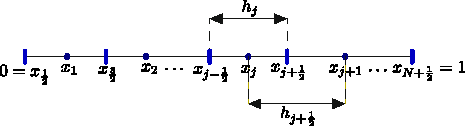
\includegraphics[width=.4\paperwidth]{fv1d}
		\caption{Malla de volúmenes finitos $1$D de
			$\Omega=\left(0,1\right)$.
			Los nodos de índices fraccionarios
			\begin{math}
				{\big\{x_{j\pm\frac{1}{2}}\big\}}^{N}_{j=1}
			\end{math}
			son los extremos de las celdas
			\begin{math}
				\Omega_{j}=
				\big[
					x_{j-\frac{1}{2}},
					x_{j+\frac{1}{2}}
					\big]
			\end{math}
			cuyo tamaño es $h_{j}$, y los nodos de índices enteros
			\begin{math}
				{\big\{x_{j}\big\}}^{N}_{j=1}
			\end{math}
			son los centros de las celdas.
		}
	\end{figure}

	Integra la EDP~\eqref{eq:PoissonBVP} en $\Omega_{j}$ y emplea
	el teorema fundamental del cálculo, obtenga
	\begin{equation}\label{eq:PoissonBVPIntegral}
		\forall j=1,\dotsc,N:
		-\diff{u}{x}[x_{j+\frac{1}{2}}]+
		\diff{u}{x}[x_{j-\frac{1}{2}}]=
		-\int_{\Omega_{j}}
		\diff[2]{u\left(x\right)}{x}
		\dl x=
		\int_{\Omega_{j}}
		f\left(x\right)\dl x.
	\end{equation}

	\note{
		Emplee el Teorema del valor medio para integrales definidas y
		aproxime los flujos numéricos en la interfaz como la diferencia
		de promedio entre dos celdas adyacentes, dividido entre la
		distancia de los centros de esas celdas.
	}
\end{frame}

\begin{frame}
	\frametitle{\secname}

	\begin{align}
		\shortintertext{
			Sea
			\begin{math}
				h=
				\max
				\left\{
				h_{j}\mid 0\leq j\leq N
				\right\}
			\end{math}
			y dado que
			\begin{math}
				u\in
				C^{2}\left(\Omega\right)
			\end{math},
			por el teorema de Taylor en la celda $\Omega_{j}$ se tiene
		}\label{eq:Taylor}
		\forall j=1,\dotsc,N:
		u\big(x_{j+\frac{1}{2}}\big)+
		\big(x-x_{j+\frac{1}{2}}\big)
		\diff{u}{x}[x_{j+\frac{1}{2}}]+
		\mathcal{O}\big(h^{2}\big)   & =
		u\left(x\right).
		\uncover<2->{
		\shortintertext{
		Use la condición de frontera $u\big(x_{\frac{1}{2}}\big)=0$
		en~\eqref{eq:Taylor} e integre sobre $\Omega_{1}$.
		}
		{\bigg[
		\frac{x^{2}}{2}-x_{\frac{1}{2}}x
		\bigg]}^{x_{\frac{3}{2}}}_{x_{\frac{1}{2}}}
		\diff{u}{x}[x_{\frac{1}{2}}]
		\dl x+
		\mathcal{O}\big(h^{3}\big)   & =
		\int_{\Omega_{1}}
		u\left(x\right)
		\dl x.\notag                              \\
		\diff{u}{x}[x_{\frac{1}{2}}] & \approx
		\frac{1}{h_{\frac{1}{2}}}
		\left[
			\frac{1}{h_{1}}
			\int_{\Omega_{1}}
			u\left(x\right)
			\dl x
			\right].\notag
		% 	\forall j=1,\dotsc,N-1:
		% \diff{u}{x}[x_{j+\frac{1}{2}}] & \approx
		% 	\frac{1}{h_{j+\frac{1}{2}}}
		% 	\left[
		% 		\frac{1}{h_{j+1}}
		% 		\int_{\mathclap{\Omega_{j+1}}}
		% 		u\left(x\right)
		% 		\dl x-
		% 		\frac{1}{h_{j}}
		% 		\int_{\Omega_{j}}
		% 		u\left(x\right)
		% 		\dl x
		% \right].\notag                           \\
		% \diff{u}{x}[x_{N+\frac{1}{2}}] & \approx
		% 	-\frac{1}{h_{N+\frac{1}{2}}}
		% 	\left[
		% 		\frac{1}{h_{N}}
		% 		\int_{\Omega_{N}}
		% 		u\left(x\right)
		% 		\dl x
		% 		\right].\notag
		}
		\shortintertext{
			Integre~\eqref{eq:Taylor} en $\Omega_{j}$,
		}
		\forall j=0,\dotsc,N:
		u\big(x_{j+\frac{1}{2}}\big)h_{j}+
		\diff{u}{x}[x_{j+\frac{1}{2}}]
		\int_{\Omega_{j}}
		\big(x-x_{j+\frac{1}{2}}\big)
		\dl x+
		\mathcal{O}\big(h^{3}\big)   & =
		\int_{\Omega_{j}}
		u\left(x\right)
		\dl x.\notag
		% \uncover<2->{
		% 	\shortintertext{
		% 		En $j=0$, la condición de frontera es
		% 		$u\big(x_{\frac{1}{2}}\big)=0$.
		% 	}
		% 	u\big(x_{\frac{1}{2}}\big)+
		% 	\frac{h_{1}}{2}
		% 	\diff{u}{x}[x_{\frac{1}{2}}]+
		% 	\mathcal{O}\big(h^{2}\big)=
		% 	\frac{1}{h_{1}}
		% 	\int_{\Omega_{1}}
		% 	u\left(x\right)
		% \dl x                                                                                     & \implies
		% 	\left|
		% 	\frac{1}{h_{\frac{1}{2}}}
		% 	\left[
		% 		\frac{1}{h_{1}}
		% 		\int_{\Omega_{1}}
		% 		u\left(x\right)
		% 		\dl x
		% 		\right]-
		% 	\diff{u}{x}[x_{\frac{1}{2}}]
		% 	\right|\leq
		% 	Ch.\notag
		% }
		% \uncover<3->{
		% 	\shortintertext{
		% 		Para $j=1,\dotsc,N-1$, en las celdas $\Omega_{j}$ y
		% 		$\Omega_{j+1}$.
		% 	}
		% \begin{aligned}
		% 		u\big(x_{j+\frac{1}{2}}\big)-
		% 		\frac{h_{j}}{2}
		% 		\diff{u}{x}[x_{j+\frac{1}{2}}]+
		% 		\mathcal{O}\big(h^{2}\big) & =
		% 		\frac{1}{h_{j}}
		% 		\int_{\Omega_{j}}
		% 		u\left(x\right)
		% 		\dl x                          \\
		% 		u\big(x_{j+\frac{1}{2}}\big)+
		% 		\frac{h_{j+1}}{2}
		% 		\diff{u}{x}[x_{j+\frac{1}{2}}]+
		% 		\mathcal{O}\big(h^{2}\big) & =
		% 		\frac{1}{h_{j+1}}
		% 		\int_{\mathclap{\Omega_{j+1}}}
		% 		u\left(x\right)
		% 		\dl x
		% 	\end{aligned} & \implies
		% 	\left|
		% 	\frac{1}{h_{j+\frac{1}{2}}}
		% 	\left[
		% 		\frac{1}{h_{j+1}}
		% 		\int_{\mathclap{\Omega_{j+1}}}
		% 		u\left(x\right)
		% 		\dl x-
		% 		\frac{1}{h_{j}}
		% 		\int_{\Omega_{j}}
		% 		u\left(x\right)
		% 		\dl x
		% 		\right]
		% 	-\diff{u}{x}[x_{j+\frac{1}{2}}]
		% 	\right|\leq
		% 	Ch.\notag
		% }
		% \uncover<4->{
		% 	\shortintertext{
		% 		En $j=N$, la condición de frontera es
		% 		$u\big(x_{N+\frac{1}{2}}\big)=0$.
		% 	}
		% 	u\big(x_{N+\frac{1}{2}}\big)+
		% 	\frac{h_{N}}{2}
		% 	\diff{u}{x}[x_{N+\frac{1}{2}}]+
		% 	\mathcal{O}\big(h^{2}\big)=
		% 	\frac{1}{h_{N}}
		% 	\int_{\Omega_{N}}
		% 	u\left(x\right)
		% \dl x                                                                                     & \implies
		% 	\left|
		% 	\frac{1}{h_{N+\frac{1}{2}}}
		% 	\left[
		% 		\frac{1}{h_{N}}
		% 		\int_{\Omega_{N}}
		% 		u\left(x\right)
		% 		\dl x
		% 		\right]-
		% 	\diff{u}{x}[x_{N+\frac{1}{2}}]
		% 	\right|\leq
		% 	Ch.
		% }\notag
		\shortintertext{
			Defina los flujos numéricos que aproximan los flujos
			$-\diff{u}{x}[x_{j+\frac{1}{2}}]$ y la integral sobre la
			celda el término fuente.
		}
		F_{\frac{1}{2}}              & \coloneqq
		-\frac{u_{1}}{h_{\frac{1}{2}}}.           \\
		\forall j=2,\dotsc,N-1:
		F_{j+\frac{1}{2}}            & \coloneqq
		-\frac{u_{j+1}-u_{j}}{h_{j+\frac{1}{2}}}. \\
		F_{N+\frac{1}{2}}            & \coloneqq
		-\frac{u_{N}}{h_{N+\frac{1}{2}}}.
	\end{align}
\end{frame}

\begin{frame}
	\frametitle{\secname}

	\begin{align*}
		\uncover<2->{
			\shortintertext{
				Reemplace en~\eqref{eq:PoissonBVPIntegral} y obtenga el
				esquema de volúmenes finitos
			}
			\forall j=1,\dotsc,N:
			F_{j+\frac{1}{2}}-
		F_{j-\frac{1}{2}}                   & =
			f_{j}\coloneqq
			\int_{\Omega_{j}}
			f\left(x\right)
			\dl x.
		}
		\uncover<3->{
		\shortintertext{
			Reescriba el esquema línea por línea,
		}
		\left(
		\frac{1}{h_{\frac{1}{2}}}+\frac{1}{h_{\frac{3}{2}}}
		\right)
		u_{1}-
		\frac{u_{2}}{h_{\frac{3}{2}}}=
		F_{\frac{3}{2}}-F_{\frac{1}{2}}     & =
		f_{1}.                                  \\
		\forall j=2,\dotsc,N-1:
		-\frac{u_{j-1}}{h_{j-\frac{1}{2}}}+
		\left(
		\frac{1}{h_{j-\frac{1}{2}}}+
		\frac{1}{h_{j+\frac{1}{2}}}
		\right)
		u_{j}-
		\frac{u_{j+1}}{h_{j+\frac{1}{2}}}=
		F_{j+\frac{1}{2}}-F_{j-\frac{1}{2}} & =
		f_{j}.                                  \\
		-\frac{u_{N-1}}{h_{N-\frac{1}{2}}}+
		\left(
		\frac{1}{h_{N-\frac{1}{2}}}+
		\frac{1}{h_{N+\frac{1}{2}}}
		\right)
		u_{N}=
		F_{N+\frac{1}{2}}-F_{N-\frac{1}{2}} & =
		f_{N}.
		}
	\end{align*}
\end{frame}

\begin{frame}
	Note que
	\begin{align*}
		\begin{bmatrix}
			\dfrac{1}{h_{\frac{1}{2}}}+\mathcolor{red}{\mathcolor{red}{\dfrac{1}{h_{\frac{3}{2}}}}} & -\mathcolor{red}{\dfrac{1}{h_{\frac{3}{2}}}}                                              & 0                                                 & \cdots                                                                                          & 0                                                                           \\
			-\mathcolor{red}{\dfrac{1}{h_{\frac{3}{2}}}}                                            & \mathcolor{red}{\dfrac{1}{h_{\frac{3}{2}}}}+\mathcolor{PineGreen}{\dfrac{1}{h_{\frac{5}{2}}}} & -\mathcolor{PineGreen}{\dfrac{1}{h_{\frac{5}{2}}}}    & \ddots                                                                                          & \vdots                                                                      \\
			0                                                                                       & -\mathcolor{PineGreen}{\dfrac{1}{h_{\frac{5}{2}}}}                                            & \ddots                                            & \ddots                                                                                          & 0                                                                           \\
			0                                                                                       & \ddots                                                                                    & \ddots                                            & -\mathcolor{orange}{\dfrac{1}{h_{N-\frac{3}{2}}}}                                               & 0                                                                           \\
			\vdots                                                                                  & \ddots                                                                                    & -\mathcolor{orange}{\dfrac{1}{h_{N-\frac{3}{2}}}} & \mathcolor{orange}{\dfrac{1}{h_{N-\frac{3}{2}}}}+\mathcolor{blue}{\dfrac{1}{h_{N-\frac{1}{2}}}} & -\mathcolor{blue}{\dfrac{1}{h_{N-\frac{1}{2}}}}                             \\
			0                                                                                       & \cdots                                                                                    & 0                                                 & -\mathcolor{blue}{\dfrac{1}{h_{N-\frac{1}{2}}}}                                                 & \mathcolor{blue}{\dfrac{1}{h_{N-\frac{1}{2}}}}+\dfrac{1}{h_{N+\frac{1}{2}}}
		\end{bmatrix}
		\begin{bmatrix}
			u_{1}   \\
			u_{2}   \\
			\vdots  \\
			\vdots  \\
			\vdots  \\
			\vdots  \\
			\vdots  \\
			\vdots  \\
			u_{N-1} \\
			u_{N}
		\end{bmatrix} & =
		\begin{bmatrix}
			f_{1}   \\
			f_{2}   \\
			\vdots  \\
			\vdots  \\
			\vdots  \\
			\vdots  \\
			\vdots  \\
			\vdots  \\
			f_{N-1} \\
			f_{N}
		\end{bmatrix}.      \\
		A^{h}U^{h}      & =
		F^{h}.
	\end{align*}

	\pause

	\begin{theorem}[El sistema $A^{h}U^{h}=F^{h}$ tiene solución~\cite{Thomas1999}]
		La matriz $A^{h}\in\mathbb{R}^{N\times N}$ es simétrica definida
		positiva, y por lo tanto invertible.
	\end{theorem}

	\pause

	\begin{proof}
		\begin{equation*}
			\forall x\in\mathbb{R}^{N}\setminus\left\{0\right\}:
			x^{T}A^{h}x=
			\sum_{j=1}^{N}
			x_{j}
			\mathcolor{DarkBlue}{
				{\big(A^{h}x\big)}_{j}
			}=
			\sum_{j=1}^{N}
			x_{j}
			\mathcolor{DarkBlue}{
				\left[
					\frac{1}{h_{j}}
					\left(
					-\frac{x_{j+1}-x_{j}}{h_{j+\frac{1}{2}}}+
					\frac{x_{j}-x_{j-1}}{h_{j-\frac{1}{2}}}
					\right)
					\right]
			}=
			\frac{x^{2}_{1}}{h_{\frac{1}{2}}}+
			\sum_{j=1}^{N-1}
			\frac{{\left(x_{j+1}-x_{j}\right)}^{2}}{h_{j+\frac{1}{2}}}+
			\frac{x^{2}_{N}}{h_{N+\frac{1}{2}}}
			>0.
		\end{equation*}
	\end{proof}
\end{frame}

% \begin{frame}
% 	El error de truncamiento es
% 	\begin{align*}
% 		h_{j}
% 		\varepsilon_{h}
% 		{\left(u\right)}_{j} & =
% 		-\frac{u\left(x_{j-1}\right)}{h_{j-\frac{1}{2}}}+
% 		\left(
% 		\frac{1}{h_{j-\frac{1}{2}}}+\frac{1}{h_{j+\frac{1}{2}}}
% 		\right)
% 		u\left(x_{j}\right)-
% 		\frac{u\left(x_{j+1}\right)}{h_{j+\frac{1}{2}}}-
% 		f_{j}.                   \\
% 		\varepsilon_{h}
% 		{\left(u\right)}_{j} & =
% 		\left[
% 			1-
% 			\frac{1}{2h_{j}}
% 			\left(
% 			h_{j-\frac{1}{2}}+
% 			h_{j+\frac{1}{2}}
% 			\right)
% 			\right]
% 		\diff[2]{u}{x}[x_{j}]+
% 		\mathcal{O}\left(h\right).
% 	\end{align*}

% \begin{theorem}
% 	Sea $\Omega=\left(0,1\right)$.
% 	Si $f\in C^{0}\big(\overline{\Omega}\big)$, entonces
% 	$\exists C>0$ que no depende de $h$ tal que
% 	\begin{math}
% 		\max\limits_{1\leq j\leq N}
% 		\left|
% 		u_{j}-
% 		\frac{1}{h_{j}}
% 		\int_{\Omega_{j}}
% 		u\left(x\right)\dl x
% 		\right|=
% 		\max\limits_{1\leq j\leq N}
% 		\left|
% 		u_{j}-
% 		u\left(x_{j}\right)
% 		\right|\leq
% 		Ch
% 	\end{math}.
% \end{theorem}

% \begin{proof}
% 	Defina
% 	\begin{align*}
% 		e_{0}                        & =0. \\
% 		\forall j=1,\dotsc,N:
% 		e_{n}                        & =
% 		u_{n}-\frac{f_{j}}{h_{j}}.         \\
% 		e_{N+1}                      & =0. \\
% 		\forall j=1,\dotsc,N:
% 		\overline{F}_{j+\frac{1}{2}} & =
% 		-\diff{u}{x}[x_{j+\frac{1}{2}}].
% 	\end{align*}
% \end{proof}
% \end{frame}

% \subsection{Implementación del método de volúmenes finitos}

% \begin{frame}
% 	% https://www.sci-hub.in/10.1016/s1570-8659(00)07005-8#page=21
% 	% https://hal.science/hal-02100732v2/document
% 	% https://www.i2m.univ-amu.fr/perso/raphaele.herbin/PUBLI/anedp.pdf
% 	% https://www.i2m.univ-amu.fr/perso/thierry.gallouet/tele.d/anum.d/envoi1.pdf
% 	\begin{theorem}[]
% 		Sea $\Omega=\left(0,1\right)$.
% 		Si $f\in C\big(\overline{\Omega}\big)$ y
% 		$u\in C^{2}\big(\overline{\Omega}\big)$, entonces
% 		$\exists\,!U^{h}\in\mathbb{R}^{N}$ que es solución
% 		y $\exists C>0$ que solo depende de $u$ tal que
% 		\begin{equation*}
% 			\sum_{j=0}^{N}
% 			\frac{\left(e_{j+1}-e_{j}\right)^{2}}{h_{j+\frac{1}{2}}}\leq
% 			C^{2}h^{2}.
% 		\end{equation*}
% 	\end{theorem}

% 	\begin{example}[{\cite[p.~15]{Frey2008}}]
% 		Considere el problema de valor de frontera Sea
% 		\begin{math}
% 			f\left(x\right)=
% 			\frac{\pi^{2}}{4}
% 			\cos\left(\frac{\pi x}{2}\right)
% 		\end{math}
% 		y considere una malla de $\left(-1,1\right)$.
% 		La solución exacta es
% 		\begin{math}
% 			u\left(x\right)=
% 			\cos\left(\frac{\pi x}{2}\right)
% 		\end{math}.
% 	\end{example}
% \end{frame}
